%%%%%%%%%%%%%%%%%%%%%%%%%%%%%%%%%%%%%%%%%%%%%%%%%
%%%%%%%%%%%%%%%%%%%%%%%%%%%%%%%%%%%%%%%%%%%%%%%%%

\chapter{Experimental Setup}
\label{chap:third}

%%%%%%%%%%%%%%%%%%%%%%%%%%%%%%%%%%%%%%%%%%%%%%%%%
%%%%%%%%%%%%%%%%%%%%%%%%%%%%%%%%%%%%%%%%%%%%%%%%%

This chapter details the experimental setup for the simulations that were performed. The parameters used in the experiment are explained in Section~\ref{parameters}, while Section~\ref{thri:third:performancemeasures} defines the performance measures used to evaluate the results of the experiment. Finally, section~\ref{thri:third:environmenttypes} discusses the environment types and how they have been generated, and the process is summarized in Section~\ref{third:summary}

%%%%%%%%%%%%%%%%%%%%%%%%%%%%%%%%%%%%%%%%%%%%%%%%%
%%%%%%%%%%%%%%%%%%%%%%%%%%%%%%%%%%%%%%%%%%%%%%%%%

%Parameter
\section{Parameters}
\label{parameters}

For each class of environment, the following configurations were tested: The environment grid size, $S=50,100,200,300, 500$ where $S$ is the width and length of the grid and the percentage of the grid covered by items $p$, where $p= 0.05\%$, $0.2\%$, $0.5\%$, $0.7\%$, $0.9\%$. The ratio of prioritized to non-prioritized items $r$, is varied, where $r=0$, $0.2$,$0.25$, $0.333$, $0.5$, $0.667$, $0.75$, $0.8$, $1$. Honey bee specific parameters were selected based on \cite{seeley2009wisdom} as 
$t_{max}=200$ time steps, $f_{max}=100$ time steps, $\phi=0.8$ and $\rho=0.1$.

For all algorithms, robots were initially configured to forage either the prioritized item or the non-prioritized item with a ratio of $\tau=0$, $0.2$, $0.25$, $0.333$, $0.5$, $0.667$, $0.75$, $0.8$,$1$. The density of robots, $c$, is defined as the percentage of cells of the grid size $S$ (the length of the side of an environment) that are occupied by robots, where $c=0.1, 0.3, 0.5, 0.7, 1$.

All agents begin at random positions adjacent to the sink in the exploration state. All algorithms were run for 10000 time steps, where an agent can move maximum 1 grid cell at a time, to any adjacent cell not occupied by another robot or item. For all algorithms, the agents begin randomly positioned next to the sink. The beacon locating of the sinks is simulated by each agent evaluating and moving up a light intensity gradient. The colour of the light is used to distinguish between the 2 sinks.

\section{Performance Measures}
\label{thri:third:performancemeasures}

%What do I need to add to 
%TODO: The idea is to add more robots foraging the prioritized items.
The following performance measures were used: 

	\begin{itemize}
		\item	The percentage of prioritized items foraged over time,  $\sigma$ 
		\item	The percentage of non-prioritized items foraged over time, $\mu$
		\item   The average time spent by agents waiting at the sink, $\epsilon$
	\end{itemize}
	
Future studies could include the average time taken by a robot to forage an item, the average distance moved by a robot and a measure to explain the randomness of a robots movement. 
%%%%%%%%%%%%%%%%%%%%%%%%%%%%%%%%%%%%%%%%%%%%%%%%%

\section{Environment Types}
\label{thri:third:environmenttypes}
Each environment type was chosen to examine specific capabilities of the algorithms. Four different classes of environments were randomly generated as follows:
\begin{enumerate}
\item Environments where items of each type are uniformly distributed (Fig \ref{fig:uniformenv}). The uniformly distributed environment is used as a base line to test the algorithms.
\item Clustered environments have clusters of item types generated by randomly relabelling the items in clusters that are generated by Lumer-Faieta ant cemetery clustering \cite{lumer1994diversity} as either prioritized or non-prioritized items (Fig \ref{fig:clusterenv}). These algorithms test the algorithms ability to exploit item rich areas. It will also test how effectively an agent can navigate around non-prioritized items. 
\item Vein environments resemble the patterns observed in naturally occurring gold \cite{frimmel2002recent} (Fig \ref{fig:veinenv}). The vein environments will test whether an agents of a specific algorithm can take advantage of the tunnel created by foraging items in the vein. 
\item Gaussian environments have prioritized items focused around the environment center in a gaussian distribution and the non-prioritized item conversely placed in the inverse distribution. (Fig \ref{fig:gaussianenv}). The gaussian environments are used to specifically examine how an algorithm can deal with moving past non-prioritized items to reach prioritized items. 
\end{enumerate} 

\vspace{-2em}
\begin{figure} [h]
        \centering
        \begin{subfigure}[b]{0.21\textwidth}
                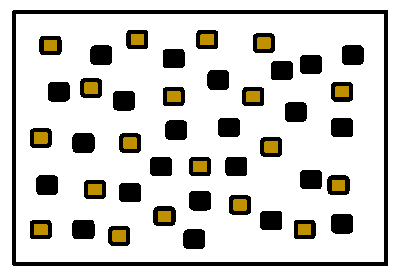
\includegraphics[width=\textwidth]{chapters/chapter4/figures/uniformenv.pdf}
                \caption{Uniform}
                \label{fig:uniformenv}
        \end{subfigure}%
        \begin{subfigure}[b]{0.205\textwidth}
                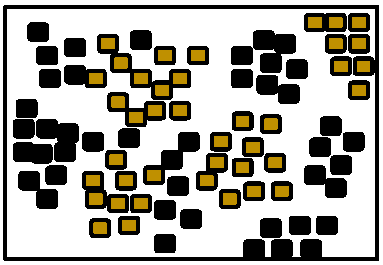
\includegraphics[width=\textwidth]{chapters/chapter4/figures/clusterenv.pdf}
                \caption{Clustered}
                \label{fig:clusterenv}
        \end{subfigure}
        \begin{subfigure}[b]{0.2\textwidth}
                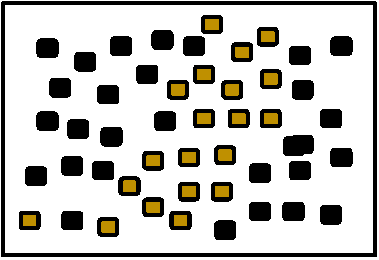
\includegraphics[width=\textwidth]{chapters/chapter4/figures/veinenv.pdf}
                \caption{Vein}
                \label{fig:veinenv}
        \end{subfigure}  
        \begin{subfigure}[b]{0.2\textwidth}
                        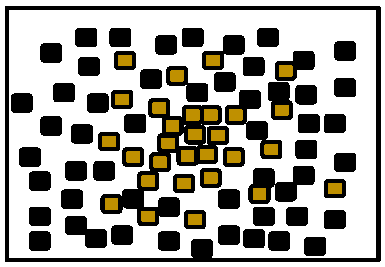
\includegraphics[width=\textwidth]{chapters/chapter4/figures/gaussianenv}
                        \caption{Gaussian}
                        \label{fig:gaussianenv}
       \end{subfigure}
        \caption{Environment Classes}\label{fig:environments}
\end{figure}

%%%%%%%%%%%%%%%%%%%%%%%%%%%%%%%%%%%%%%%%%%%%%%%%%
%%%%%%%%%%%%%%%%%%%%%%%%%%%%%%%%%%%%%%%%%%%%%%%%%

\section{Robots}
\label{chap:robots}

Foraging robots occur in all shapes, sizes and capabilities. Some robots have powerful GPS capabilities and advanced long distance sensors, and others are much simpler. This chapter defines the capabilities of the simulated robots to be used in this study. The robots are described in Section~\ref{robotdescription}, while Section~\ref{robots:obstacleavoidance} outlines the navigational capabilities of the robots. Section~\ref{simulator} discusses the simulator used and the chapter is summarized in Section~\ref{robots:summary}.

\subsection{Robot Description}
\label{robotdescription}

The artificial robots modelled in this study are based on e-puck robots \cite{mondada2009puck}, adapted with grippers. A robot is equipped with a 360 degree camera to identify objects around the robot, as well as eight local distance sensors spaced equally around the circular perimeter of the robot. Both camera and distance sensors have a depth of view of five times the robot's size. Robots use local communication which can occur in a radius of five times the robot's size. On real robots, the local communication could occur via use of light signals or ZigBee communications. The sensor and communication range is sufficiently localized with respect to the size of the environment. A robot can forage a single item at a time. The robots do not have a global positioning system (GPS) capability to locate items to position themselves in the environment. A robot cannot see an item hidden by another item. As a result robots have to explore the environment to find the prioritized items.

\subsection{Navigation and Obstacle Avoidance}
\label{navigationandobstacleavoidance}

The environments used in the simulation are of various levels of complexity: Some environments are very sparse while others have large zones of items that must be navigated around. Due to the environmental complexity, an advanced navigation and obstacle avoidance technique is required. 

The experiments in this thesis use a navigation and obstacle avoidance technique inspired by an approach developed for communication congestion avoidance in wireless sensor networks\cite{antoniou2012congestion}. Antoniou et al. use inspiration from the flocking behaviour of birds, in order to efficiently route messages around communication congestion in wireless sensor networks. In flocking behaviour of birds, birds are attracted by a global magnetic attractor to the birds final destination, while a local attractor pulls flocking birds away from areas of congestion. In the congestion avoidance algorithm, the final destination of the message being sent on the wireless sensor network is the global attractor while a local attractor pulls the message around congested areas.

The described congestion avoidance technique has been adapted to form a simple but effective navigation and obstacle avoidance technique. Robots are pulled to a global attractor which is the intended destination, while a local attractor directs robots away from local obstacles while maintaining a course to the destination.

Figure \ref{fig:obstacleavoidance} illustrates the navigation and obstacle avoidance method used by the robots. The navigation and obstacle avoidance algorithm achieves the effect of the global attractor by setting the robots field of view towards the direction to the desired destination. The destination is determined by a homing beacon or by the robot's path integration vector. The direction at the centre of the field of view is the direction to the destination. 

The effect of the local attractor is modelled by evaluating a function for each direction in the field of view, in order to select the most desirable direction. Desirability, $d$, of a direction, $i$, is defined as a path that achieves an adequate balance between clarity of the path and directness of the direction to the destination. The clarity,  $c_i$, in a particular direction $i$, is a normalized reading from the proximity sensor or camera such that $c_i\in[0,1]$. Clarity indicates the distance of next nearest obstacle such that the existence of no obstacles for the depth of view $v$ results in a value of 0 and the existance of an obstacle immediately next to the robot results in a clarify of 1, $c_i=1$. The directness of a direction $i$, $\iota_i\in[0,1]$ is calculated as the angular deviation from the direction of the destination, where a directness value of 0 is achieved when the direction $i$ is the same as direction to the destination and a directness value of 1 occurs when the direction is at the edge of the field of view, $f$. Desirability $d_i$ of direction $i$ is defined mathematically in Equation \ref{eq:1}.

\begin{equation}
	d_i= \lambda c_i + (1 - \lambda)\tau_i \\
	\label{eq:1}
\end{equation} where $\lambda$ determines whether clarity, $c_i$ or directness, $\tau_i$ of direction $i$, has more effect on desirability
. The described navigation and obstacle avoidance technique is used with all algorithms in the experiment and for algorithms $\lambda$ is set to 0.5.

\begin{figure}
	\centering
	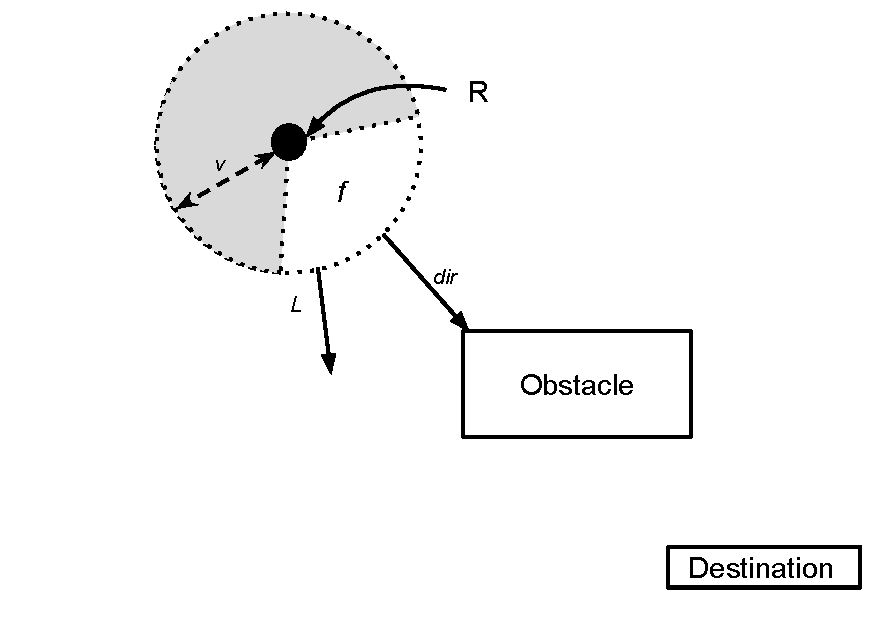
\includegraphics[width=0.75\textwidth]{chapters/chapter5/figures/ObstacleAvoidance.pdf}
	\caption{Navigation and Obstthe acle Avoidance, where $v$ is depth of view, $f$ is the field of view, $R$ is the robot, $dir$ is the direction of the destination and $L$ is a possible value of local attractor}
	\label{fig:obstacleavoidance}
\end{figure}


%%%%%%%%%%%%%%%%%%%%%%%%%%%%%%%%%%%%%%%%%%%%%%%%%
%%%%%%%%%%%%%%%%%%%%%%%%%%%%%%%%%%%%%%%%%%%%%%%%%
\subsection{Simulator}
\label{simulator}
A spatially discrete 2-dimensional grid world simulator has been developed and used in this thesis in order to accelerate computation \cite{sugawara2002swarming}. In real root experiments, algorithm performance is sensitive to the amount of time taken to load items and manoeuvre the robots \cite{ostergaard2001emergent}. The 2-dimensional grid world simulator allows for movement and loading time to be standardized across all algorithms for effective comparison.

The simulation robots function as follows:
\begin{itemize}
	\item Each robot fits into one grid block and each item takes up one grid block. 
	\item Only one item or robot can occupy a grid block at a time, which will allow for collisions and congestion to occur. 
	\item Each robot can move to an adjacent cell in any direction.
	\item Robots can load, transport and offload a single item at a time.
	\item If a robot does not pick up an item, the item forms an obstacle that must be navigated around.
\end{itemize}

The prioritized and non-prioritized sinks were placed next to each other, on a single side of the environment. The sinks were marked by light beacons that all robots can detect and navigate towards. The reason the sinks were not placed in the centre of the environment as is commonly found in swarm robotics research \cite{labella2006division} is because the original prioritized foraging problem was inspired by the use of robots to forage gold and waste in mining tunnels. A mining tunnel has a single entrance where the gold and waste must be moved to, in order to be transported to the surface \cite{brune2010extracting}. Since there is only a single entrance at the beginning of a tunnel, the sinks need to occur at the beginning of the tunnel so that the items can be easily exported.


%%%%%%%%%%%%%%%%%%%%%%%%%%%%%%%%%%%%%%%%%%%%%%%%%
%%%%%%%%%%%%%%%%%%%%%%%%%%%%%%%%%%%%%%%%%%%%%%%%%
\subsection{Summary}
\label{robots:summary}
The robots used in this study are based on that of the e-puck robots, but with gripper capabilities. The robots used a navigation and obstacle avoidance technique based on the flocking behaviour of birds where a global attractor force attracts the robot in a specific direction, while the local attractor force guide the robot around localized obstacles. A simple 2-dimensional grid-based simulator is used. Only a single robot or item could occupy a single grid cell at once, resulting in interference between robots and items. The item sinks were placed at the same end of the environment, since this research was inspired by a gold mining scenario where the robots would inhabit a tunnel with only one exit.

%%%%%%%%%%%%%%%%%%%%%%%%%%%%%%%%%%%%%%%%%%%%%%%%%
%%%%%%%%%%%%%%%%%%%%%%%%%%%%%%%%%%%%%%%%%%%%%%%%%
%%%%%%%%%%%%%%%%%%%%%%%%%%%%%%%%%%%%%%%%%%%%%%%%%
%%%%%%%%%%%%%%%%%%%%%%%%%%%%%%%%%%%%%%%%%%%%%%%%%
\section{Summary}
\label{third:summary}

This section details the parameters chosen for the algorithms as well as the performance measures selected in order to compare various aspects of the algorithms: the different percentages of each type of item foraged as well as the time spent waiting by the sink. Lastly, the environment types that were generated for experimentation in order to test different properties of the algorithms are discussed. The environment types defined have the four following distributions: uniform distribution, Gaussian distribution, clustered distribution and vein distribution. The robots were the described in terms of the capabilities of the robots themselves, techniques used by the robots for navigation and obstacle avoidance  as well as the simulation environment used.


%%%
%%%%%%%%%%%%%%%%%%%%%%%%%%%%%%%%%%%%%%%%%%%%%%%%%
%%%%%%%%%%%%%%%%%%%%%%%%%%%%%%%%%%%%%%%%%%%%%%%%%